\chapter{Grundlagen}\label{kap:grundlagen}

%####################  CHAPTER 1: Grundlagen  #################

In vorliegendem Kapitel werden zunächst die Grundlagen 
des \Glspl{ml}, mit \Glspl{nn}, 
beschrieben. Der zweite Abschnitt wird die, in der 
Bilderkennung eingesetzen, \Glspl{cnn} näher erläutern.
Im letzten Abschnitt wird die, für die Inferenz, 
verwendete Hardware, der \textit{Neural Compute Stick 2}
von \textit{Intel} beschrieben werden.


%------------------- SECTION: Machine Learning ------------------

\section{Machine Learning}\label{sec:ml}

Beim \Gls{ml}, welches ein Teilgebiet der Computerwissenschaften
ist, geht es um die Erstellung von Algorithmen, die Zusammenhänge in 
großen Datenmengen erkennen können, ohne explizit darauf programmiert
worden zu sein.
Eine Form davon ist das \textit{Supervised Learning}, bei dem
das Programm neben den Inputdaten auch die Zugehörigen Ausgaben,
in vorm von Labels, erhält, um daraus 
Regeln für die Zusammenhänge zwischen Ein- und Ausgabe Daten
abzuleiten.
Dadurch unterscheidet sich das Vorgehen wesentlich zur Programmierung 
eines klassischen Programms, bei dem die Regeln vorarb definiert 
werden müssen, wie Abbildung \ref{fig:classic_vs_ml}
veranschauliche.
\vspace{0.5cm}

\begin{figure}[H]
    \centering
    
\tikzset{
    decision/.style={
        diamond,
        draw,
        text width=4em,
        text badly centered,
        inner sep=-1pt,
        node distance=8em
    },
    block/.style={
        rectangle,
        draw,
        text width=6em,
        %minimum widhth=6em,
        minimum height=5em,
        text centered,
        node distance=20em
    },
    arrow/.style={
        draw,
        >=latex,
        ->
    },
    textfeld/.style={
        %draw,
        text centered,
        node distance=1.5em
    }
}


\begin{tikzpicture}

    
    \node (system) [block] {Klassisches\\Programm};
    \node (system2) [block, right of=system] {Machine Learning\\Programm};

    \node [textfeld, left=of system.162] (inputs) {Daten};
    \node [textfeld, left=of system.198] (regeln) {Regeln};
    \node [textfeld, right=of system] (output) {Ausgaben};

    \node [textfeld, left=of system2.162] (inputs2) {Daten};
    \node [textfeld, left=of system2.198] (output2) {Ausgaben};
    \node [textfeld, right=of system2] (regeln2) {Regeln};
    
    \draw[arrow] (inputs) -- (system.162);
    \draw[arrow] (regeln) -- (system.198);
    \draw[arrow] (system) -- (output);
    
    \draw[arrow] (inputs2) -- (system2.162);
    \draw[arrow] (output2) -- (system2.198);
    \draw[arrow] (system2) -- (regeln2);
    

\end{tikzpicture}

    \caption{Vergleich herkömmliche- und \Gls{ml}- Programmierung}
    \label{fig:classic_vs_ml}
\end{figure}
\vspace{0.5cm}

Das Ableiten der Regeln erfolgt beim \Gls{ml} in einem 
iterativen Prozess, welcher als Training bezeichnet wird.
Dabei werden die Zusammenhänge zwischen Ein- und Ausgabe Daten 
als mathematische Funktion, die numerisch an die richtigen Werte
angenähert wird, betrachtet.

Handelt es sich um einen linearen Zusammenhang der 
Daten, spricht man von einer \textit{Regression}, 
wohingegen bei einer Kategorisierung von diskreten 
Werten von einer \textit{Klassifikation} gesprochen wird.

Weitere Formen neben dem \textit{Supervised Learning} sind das 
\textit{Unsupervised Learning}, bei dem das Programm keine Labels 
erhält, sondern diese durch das Training selber finden 
soll, oder das \textit{Reinfocement Learning}, bei dem das Programm, 
durch interaktion mit der Umwelt, bestimmte Verhaltensmuster lernt.
Da in der Bachelor Arbeit nur mit dem \textit{Supervised Learning} 
gearbeitet wurde, wird auf diese Techniken im folgenden nicht 
näher eingegangen.

%------------------- SECTION: Neuronale Netze -------------------

%\newpage
\subsection{Künstliche Neuronale Netze} \label{subsec:nn}

Für komplexe Inputdaten, wie beispielsweise Bilder, bei denen 
die einzelnen Pixelwerte die Eingaben und der Inhalt des Bildes die 
gesuchte Ausgabe darstellen, werden meistens \Glspl{nn} verwendet.
Diese sind eine Form des \Glspl{ml} und bestehen aus einer 
vielzahl an, programmatisch erzeugten künstlicher Neuronen, die 
in Schichten angeordnet, miteinander verbunden sind.

Durch unterschiedlich starke Gewichtungen der einzelnen
Verbindungen, welche auch als Gewichte bezeichnet werden, 
können, wie in Abbildung \ref{fig:nn} schematisch dargestellt ist,
zu gegebene Eingaben die richtigen Ausgaben gefunden werden.

\vspace{1cm}
\begin{figure}[H]
    \centering
    \def\svgwidth{0.85\columnwidth}
    %\footnotesize
    \begin{neuralnetwork}[height=1]
    \newcommand{\nodetextclear}[2]{}
    \newcommand{\nodetexth}[2]{$h_#2$}
    \newcommand{\nodetextx}[2]{$x_#2$}
    \newcommand{\nodetexty}[2]{$y_#2$}
    \inputlayer[count=3, bias=false, title=Input\\layer, text=\nodetextx]
    \hiddenlayer[count=4, bias=false, title=Hidden\\layer, text=\nodetexth] \linklayers
    \outputlayer[count=2, title=Output\\layer, text=\nodetexty] \linklayers
\end{neuralnetwork}
    \caption{Vereinfachte Darstellung eines Künstlichen 
    Neuronalen Netzes}
    \label{fig:nn}
\end{figure}
\vspace{1cm}

Die richtigen Einstellungen der Gewichte erfolgt dabei
in dem iterativen Trainingsprozess, welcher aus folgenden 
drei schritten besteht und in Abbildung \ref{fig:train}
schematisch dargestellt ist.

\begin{itemize}
    \item \textit{Forward Pass} Für die Inputdaten anhand,
            aktueller Gewichte, eine Schätzung für die Ausgabe treffen
    \item \textit{Fehlerbestimmung} Abweichung der gemachten Schätzung,
             zum tatsächlichen Wert, berechnen
    \item \textit{Backpropagation} Minimierung der
            Abweichung, durch Veränderung der Gewichte
\end{itemize}

\vspace{1cm}
\begin{figure}[H]
    \centering
    
\tikzstyle{process} = [rectangle, fill=blue!20, minimum width=2.5cm, minimum height=1cm, text centered, draw=black]
\tikzstyle{arrow} = [thick,->,>=stealth]

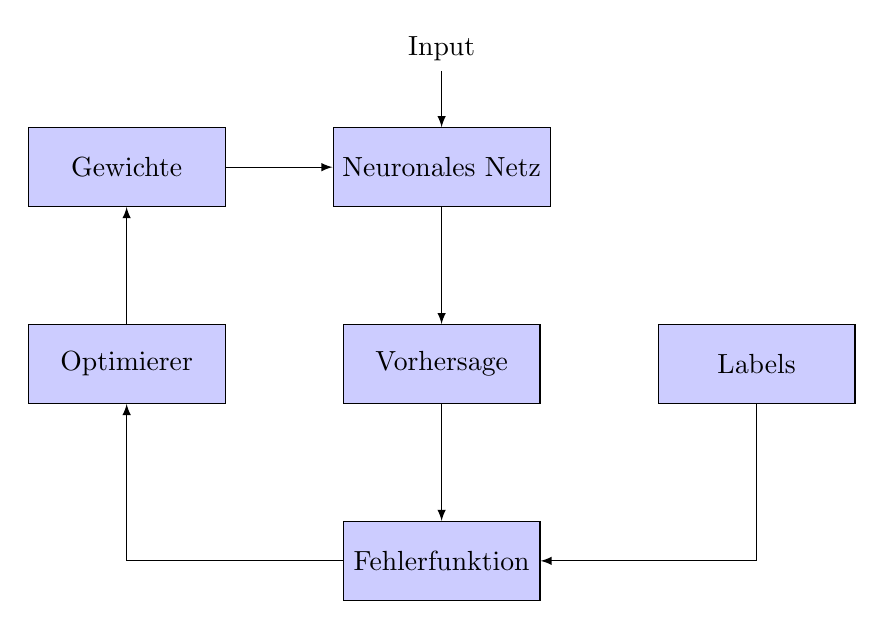
\begin{tikzpicture}[node distance=1.6cm]

  \begin{scope}[node distance=2.5cm]
    \node (nn)      [process]                   {Neuronales Netz};
    \node (pred)      [process, below of=nn]      {Vorhersage};
    \node (loss)      [process, below of=pred]      {Fehlerfunktion};
    
  \end{scope}
  
  \begin{scope}[node distance=4cm]
    \node (opt) [process, left of=pred]      {Optimierer};
    \node (weights)  [process, left of=nn] {Gewichte};
    \node (labels)   [process, right of=pred]  {Labels};
  \end{scope}

  \node (input) at (0,1.5) {Input};

  \draw[arrow] (input) -- (nn);

  \draw[arrow] (nn) -- (pred);
  \draw[arrow] (pred) -- (loss);

  \draw[arrow] (labels) |- (loss);
  \draw[arrow] (loss) -| (opt);

  \draw[arrow] (opt) -- (weights);
  \draw[arrow] (weights) -- (nn);
  
    
\end{tikzpicture}

    \caption{Schematiscer Trainingsablauf eines Neuronalen Netzes}
    \label{fig:train}
\end{figure}
\vspace{1cm}


Durch mehrfaches Durchlaufen dieser Schritte, 
kann die Fehlerfunktion soweit minimiert werden, dass 
das Modell auch für neue, ungesehene Input Daten 
richtigen Vorhersagen treffen kann.

Die Funktionsweisen der drei Schritte 
werden im folgenden näher erläutert.

\subsubsection{Forward Pass}
Im \textit{Forward Pass} werden die Eingabewerte, welche an der 
ersten Schicht aus Neuronen anliegen, durch alle Schichten hindurch 
gereicht, um in der Ausgabeschicht Schicht
das gesuchte Ergebnis zu liefern.
Dabei erhält jedes Neuron, die mit den Parametern $w_{i}$ gewichteten,
Ausgabewerte aller Neuronen der vorherigen Schicht und summiert diese
zusammen mit einem konstanten Bias Wert $b$, als Offset, auf.

Mithilfe einer Aktivierungsfunktion wird der Wert, wie 
in Abbildung \ref{fig:neuron} dargestellt ist, auf
einen bestimmten Bereich skaliert.


\vspace{1cm}
\begin{figure}[H]
    \centering
    \begin{tikzpicture}[
    % define styles    
    init/.style={ 
         draw, 
         circle, 
         inner sep=2pt,
         font=\Huge,
         join = by -latex
    },
    squa_draw/.style={ 
        draw,
        font=\Large,
        join = by -latex
    },
    squa/.style={ 
        font=\Large,
        join = by -latex
    }
]
% Top chain x1 to w1
\begin{scope}[start chain=1]
    \node[on chain=1] at (0,1.5cm)  (x1) {$x_1$};
    \node[on chain=1,join=by o-latex] (w1) {$w_1$};
\end{scope}
% Middle chain x2 to output
\begin{scope}[start chain=2]
    \node[on chain=2] (x2) {$x_2$};
    \node[on chain=2,join=by o-latex] {$w_2$};
    \node[on chain=2,init] (sigma) {$\displaystyle\Sigma$};
    \node[on chain=2,squa_draw,label=below:{\parbox{2cm}{\centering Aktivierungs\\ Funktion}}]   {$\delta(z)$};
    \node[on chain=2,squa,label=below:Output,join=by -latex] {$y_{out}$};
\end{scope}
% Bottom chain x3 to w3
\begin{scope}[start chain=3]
    \node[on chain=3,label=below:Inputs] at (0,-1.5cm) 
    (x3) {$x_3$};
    \node[on chain=3,label=below:Gewichte,join=by o-latex]
    (w3) {$w_3$};
\end{scope}
% Bias
\node[label=above:\parbox{2cm}{\centering Bias \\ $b$}] at (sigma|-w1) (b) {};
% Arrows joining w1, w3 and b to sigma
\draw[-latex] (w1) -- (sigma);
\draw[-latex] (w3) -- (sigma);
\draw[o-latex] (b) -- (sigma);

\end{tikzpicture}

% von https://medium.com/momenton/typesetting-neural-network-diagrams-with-tex-4920b6b9fc19
    \caption{Berechnungen an einem einzelnen Neuron}
    \label{fig:neuron}
\end{figure}
\vspace{1cm}

Um diesen Vorgang für eine gesamte Schicht, bestehend aus 
einer Vielzahl an Neuronen, zu berechnen, werden die Schichten 
als Vektoren $x$ und die Gewichte als Matrizen $W$ dargestellt.

Durch Bilden der Matrixmultiplikation zwischen $x$ und $W$,
 wie Gleichung \ref{eq:forward} zeigt,
erhält man den \textit{Forward Pass} von einer Schicht zur nächsten.
\vspace{0.5cm}

\begin{equation}
    \label{eq:forward}
    z = W^{T}x+b
\end{equation}
\vspace{0.5cm}

Der resultierende Vektor $z$ wird dann elementweise
einer nichtlinearen Aktivierungsfunktion $g(z)$ übergeben.

Bei dieser handelt es sich, für die mittleren Schichten, 
den sogenannten \textit{Hidden Layern},  
meist um die in Abbildung \ref{plot:relu} dargestellte
Funkton \textit{ReLU}, welche positive Werte beibehält und negative 
Werte zu 0 setzt.

In der letzten Schicht, welche die Wahrscheinlichkeiten 
für mögliche Ausgaben enthält, wird eine Aktivierungsfunktion
verwendet, die den Wert zwischen 0 und 1 skaliert.
Dabei wird für eine binären Klassifikation die 
in Abbildung \ref{plot:sigmoid} dargestellte Funktion 
\textit{Sigmoid} verwendet, welche die Werte S-Förmig zwischen 
0 und 1 skaliert.

Für eine kategorische Klassifikation, 
mit mehr als zwei möglichen Ausgabewerten, 
wird die in Gleichung 
\ref{eq:softmax} dargestellte Funktion \textit{Softmax} 
verwendet, welche eine
Wahrscheinlichkeitsverteilung über alle Werte
der Ausgebeschicht generiert.

\begin{equation}
    \label{eq:softmax}
    g(z_{i}) = \frac{e^{z_{i}}}{\sum_{j} e^{z_{j}}}
\end{equation}
\newpage
%\vspace{1cm}
\begin{minipage}{0.5\textwidth}
    \centering
    \begin{equation*}
        \label{eq:relu}
        g(z) = max\{0,z\}
    \end{equation*}
\end{minipage}
\vspace{1cm}
\begin{minipage}{0.5\textwidth}
    \centering
    \begin{equation*}
        \label{eq:sidmoid}
        g(z) = \frac{1}{1 + e^{-z}}
    \end{equation*}    
\end{minipage}
\begin{minipage}{0.5\textwidth}
    \centering
    \begin{tikzpicture}[scale=0.6]
    \begin{axis}
        %scale only axis=true,
        [
            scale only axis=true,
            width=0.8\textwidth,
            height=5cm,
            axis x line=middle,
            axis y line=center,
            tick align=outside
        ]
        
        \addplot
        [
            blue,
            mark=none,
            smooth,
            domain=-3:6
        ] 
        (x,{(x>=0)*x});

	\end{axis}
\end{tikzpicture}
    \captionof{figure}{ReLU Funktion} 
    \label{plot:relu}
\end{minipage}
\begin{minipage}{0.5\textwidth}
    \centering
    \begin{tikzpicture}[scale=0.6]
    \begin{axis}
        %scale only axis=true,
        [
            scale only axis=true,
            width=\textwidth,
            height=5cm,
            % xmin=-6,
            % xmax=6,
            axis x line=middle,
            axis y line=center,
            tick align=outside
        ]
        
        \addplot
        [
            blue,
            mark=none,
            smooth,
            domain=-6:6
        ] 
        (x,{1/(1+exp(-x))});

	\end{axis}
\end{tikzpicture}
    \captionof{figure}{Sigmoid Funktion} 
    \label{plot:sigmoid}
\end{minipage}
\vspace{1cm}


\subsubsection{Fehlerbestimmung}
Die Abweichung des geschätzten Wertes, welcher an den
Neuronen der letzten Schicht anliegt, zum tatsächlichen Wert,
wird mithilfe einer geeigneten Fehler- oder auch Lossfunktion
ermittelt.
Ein Regressionsmodell verwendet hierbei oft 
den absoluten oder quadratischen Abstand der beiden 
Werte, wohingegen für Klassifikationsmodelle meist 
der Logarithmus verwendet wird.
In Gleichung \ref{eq:crossentropy} ist die logarithmische Lossfunktion
\textit{Cross entropy}, für eine Binäre Klassifikation 
dargestellt.
Durch den Logarithmus wird der Loss um so größer,
je weiter die Schätzung $y$ vom 
tatsächlichen Wert $\hat{y}$ abweicht.
\vspace{0.5cm}

\begin{equation}
    \label{eq:crossentropy}
    L = \hat{y}log(y) + (1 - \hat{y})log(1 - y)
\end{equation}
\vspace{0.5cm}


\subsubsection{Backpropagation}

Die Anpassung der Gewichte, zur Minimierung der Lossfunktion, 
kann durch Berechnung des Gradienten dieser, erfolgen.

Dafür wird die die Fehlerfunktion $L$, für jede Schicht, partiell
nach den Gewichten $w$ der Schicht abgeleitet,
was, wie in Gleichung \ref{eq:backprop}
dargestellt, mithilfe der Kettenregel geschieht.
Mit dem ermittelten Gradienten werden
dann die Gewichte nach Gleichung \ref{eq:update_wieghts}
mit einer Schrittweite $\eta$ angepasst.
\vspace{0.5cm}

\begin{equation}
    \label{eq:backprop}
    \frac{\partial L}{\partial w} = \frac{\partial L}{\partial z}\frac{\partial z}{\partial w}
\end{equation}
\vspace{0.5cm}
\begin{equation}
    \label{eq:update_wieghts}
    w  \leftarrow w - \eta \frac{\partial L}{\partial w}
\end{equation}
\vspace{1cm}



%------------------- SUBSECTION: Validierung -------------------
\subsection{Validierung und Overfitting}\label{subsec:validation}

Um überprüfen zu können, ob und wie gut, ein Modell die Zusammenhänge
in den Trainingsdaten generalisiert hat, also auch für neue Daten
anwendbar ist, wird der Datensatz in einen Trainings- und
einen Testdatensatz aufgeteilt.

Die Abweichung wird während des Trainings für beide Datensetze 
berechnet, die Korrektur der Gewichte, mittels Backpropagation,
erfolgt jedoch nur anhand der Trainingsdaten.

Indem beide Lossfunktionen als Funktion, in Abhängigkeit 
der Iterationen, geplottet werden, kann eine Überanpassung
des Modells an die Trainingsdaten, festgestellt werden.

Dabei handelt es sich um das sogenannte \textit{\Gls{overfitting}}
was daran zu erkennen ist, das sich nur noch der Wert des 
Trainingsloss verringert und der der Testdaten 
gleich bleibt oder sich wie in Abbildung \ref{fig:overfitting}
dargestellt, wieder verschlechtert.
\vspace{1cm}

\begin{figure}[H]
    \centering
    \def\svgwidth{0.5\textwidth}
    \input{Bilder/overfitting.pdf_tex}
    \caption{Overfitting, anhand der Losskurven}
    \label{fig:overfitting}
\end{figure}
\vspace{1cm}

Gründe für das \Gls{overfitting} können sein,
dass zu wenig Trainingsdaten
verwendet wurden, oder ein, für den Anwendungsfall, 
zu komplexes Modell gewählt wurde.

Durch die Überparametrisierung eines zu komplexen Modells hat 
dieses die Möglichkeit sich an jeden Trainingsdatenpunkt einzeln
anzupassen, sodass keine Ggneralisierbaren 
Aussagen für neue Datenpunkte mehr getroffen werden können.

Der andere Extremfall ist das \textit{Underfitting}, 
bei dem das Modell, aufgrund zu weniger Parameter, nicht die 
Möglichkeit hat, sich an die Trainingsdaten anzunähern.

Die Plots in Abbildung \ref{fig:over_under_fit} veranschaulichen 
die drei Fälle anhand einer polynomialen Funktionen,
die sich an gegebene Datenpunkte, mit unterschiedlech hohem 
Grad, annähern soll.

\vspace{1cm}
\begin{figure}[H]
    \centering
    \def\svgwidth{\textwidth}
    \input{Bilder/over_under_fit.pdf_tex}
    \caption{Annäherung unterschiedlich komplexer Modelle an die gleichen 
        Datenpunkte}
    \label{fig:over_under_fit}
\end{figure}
\vspace{1cm}

Das Auftreten von Overfitting kann entweder durch 
Verwendung einer größeren Anzahl an Trainingsdaten, 
oder mit einer der Folgenden Techniken, vermieden werden.


\subsubsection{Augmentierung}

\textit{Augmentierung} der Daten ist eine effektive Technik 
gegen \Gls{overfitting}, bei der künstlich,
aus den vorhandenen Daten, mehr Daten generiert werden. 
Im Fall der Bilderkennung werden hierbei 
die Inputbilder leicht abgeändert, indem z.B. geometrische 
Transformationen oder manipulationen der Pixelwerte 
vorgenommen werden.


\subsubsection{Regularisierung der Parameter}

Bei der \textit{Regularisierung} wird der Lossfunktion,
als weiterer Term, eine Aufsummierung aller Gewichte
hinzugefügt.

Die Minimierung der Lossfunktion hat dann auf 
die Gewichte den Effekt, dass diese möglichst 
kleine Werte behalten, wodurch das Modell weniger
Möglichkeit zur Überanpassung hat.

Dabei wird zwischen der \textit{L1 Regularisierung},
mit einer absoluten, und der in Gleichung \ref{eq:regularization}
dargestellten \textit{L2 Regularisierung}, mit einer 
quadratischen Aufsummierung der
Gewichte unterschieden.

\begin{equation}
    \label{eq:regularization}
    J = L + \lambda \sum_{i} w_{i}^{2}
\end{equation}


\subsubsection{Dropout}
\textit{Dropout} ist eine Technik, bei der in einigen Schichten 
mit einer bestimmten Wahrscheinlichkeit Werte von 
Neuronen zu 0 gesetzt werden.
Dadurch wird das Modell gezwungen alternative
Gewichtsanpassungen zu finden.

\begin{figure}[H]
    \centering
    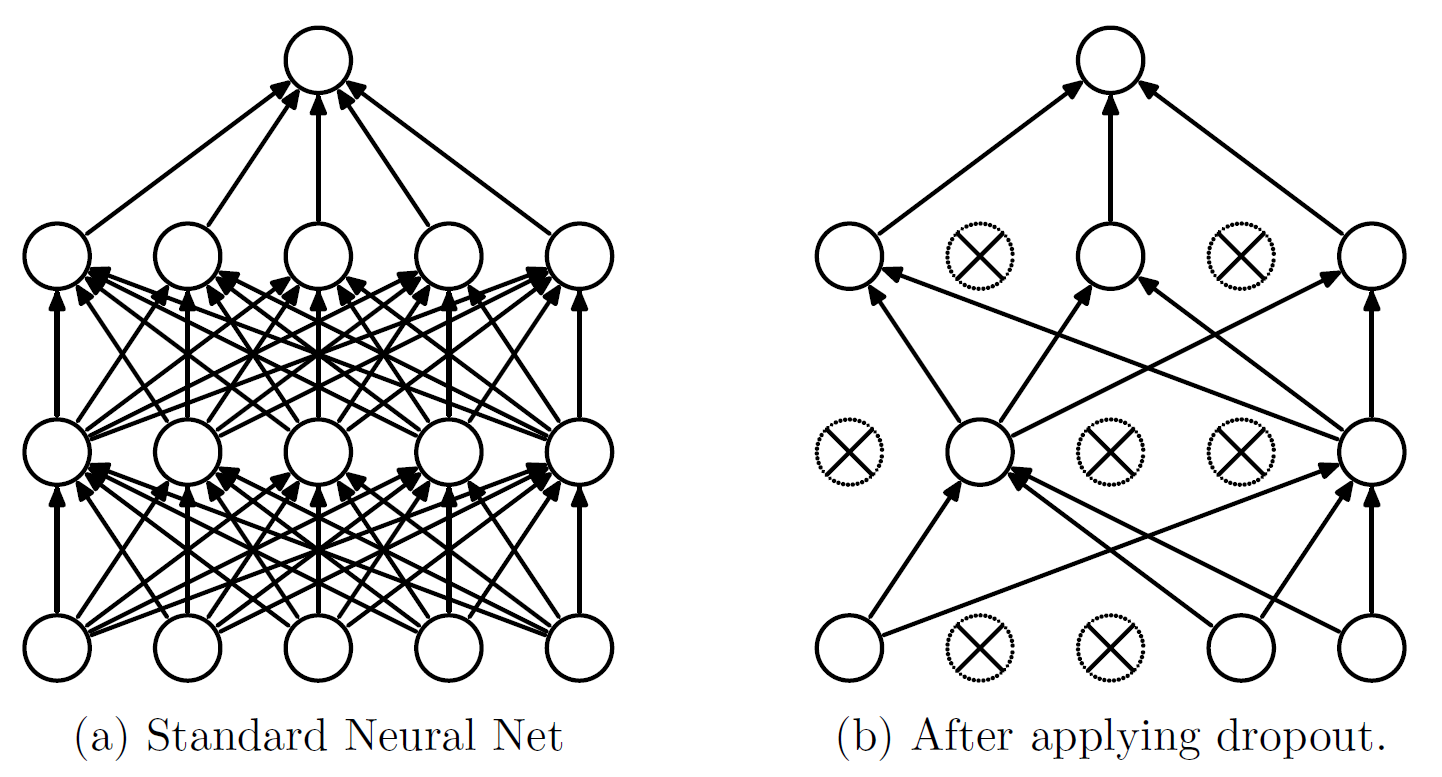
\includegraphics[width=0.6\textwidth]{dropout.png}
    \caption{Prinzip Dropout \cite{maksutovDeepStudyNot2018}}
    \label{fig:dropout}
\end{figure}


\subsubsection{Early Stopping}
Beim \textit{Early Stopping} wird das Training, 
bevor \Gls{overfitting} stattfinden kann, abgebrochen.
Das ist, wie in Abbildung \ref{fig:overfitting}
markiert, durch das Minimum der Losskurve der Testdaten 
definiert.



%------------------- SUBSECTION: ML Frameworks ---------------
\subsection{Machine Learning Frameworks}

\Gls{ml} Algorithmen beinhalten eine vielzahl an komplexen
Berechnungsschritten und Parametern. Um diese nicht jedesmal 
von Grund auf neu implementieren zu müssen 
bieten\Glspl{framework}
eine einfache Möglichkeit die Modelle zu konstruieren.

Einige der bekannten Open Source \Glspl{framework} sind
 Tensorflow, Caffe, Torch, Kaldi oder Scikit-Learn.

Für die Bachelor Arbeit wurde Tensorflow verwendet,
ein von Google stammendes \Gls{framework},
welches aufgrund seiner hohen Flexibilität besonders 
in der Forschung oft verwendet wird.



%---------------- SUBSECTION: Convolutional ----------------
\section{Convolutional Neural Networks}\label{subsec:cnn}

\Glspl{cnn} erweitern die in Abschnitt \ref{subsec:nn} beschriebenen
\Glspl{nn} um zusätzliche Schichten,
die vor der eigentliche Klassifikation ausgeführt werden
und Merkmale aus den Input Daten herausextrahieren.
Diese Schichten erhalten die Input Daten als
zweidimensionale Matrix und führen darauf 
mathematische Faltungsoperationen aus.
\Glspl{cnn} kommen größtenteils in der Bilderkennung zum 
Einsatz, weitere Anwendungsgebiete sind 
z.B. die Spracherkennung.

Anstatt das alle Neuronen zweier benachbarter Schichten 
durch gewichtete Parameter miteinander verbunden sind, 
stellen kleinere, sogenannte Filter Matrizen, die 
Parameter dar.
Diese werden zeilenweise über das Inputbild 
geschoben, wobei an jeder Stelle eine mathematische 
Faltung mit dem überlappten Bereich des Inputs 
durchgeführt wird. In Abbildung \ref{fig:faltung}
ist dieser Vorgang zur Veranschaulichung dargestellt.
\vspace{1cm}

\begin{figure}[H]
    \centering
    \begin{minipage}{0.49\textwidth}
        \centering
        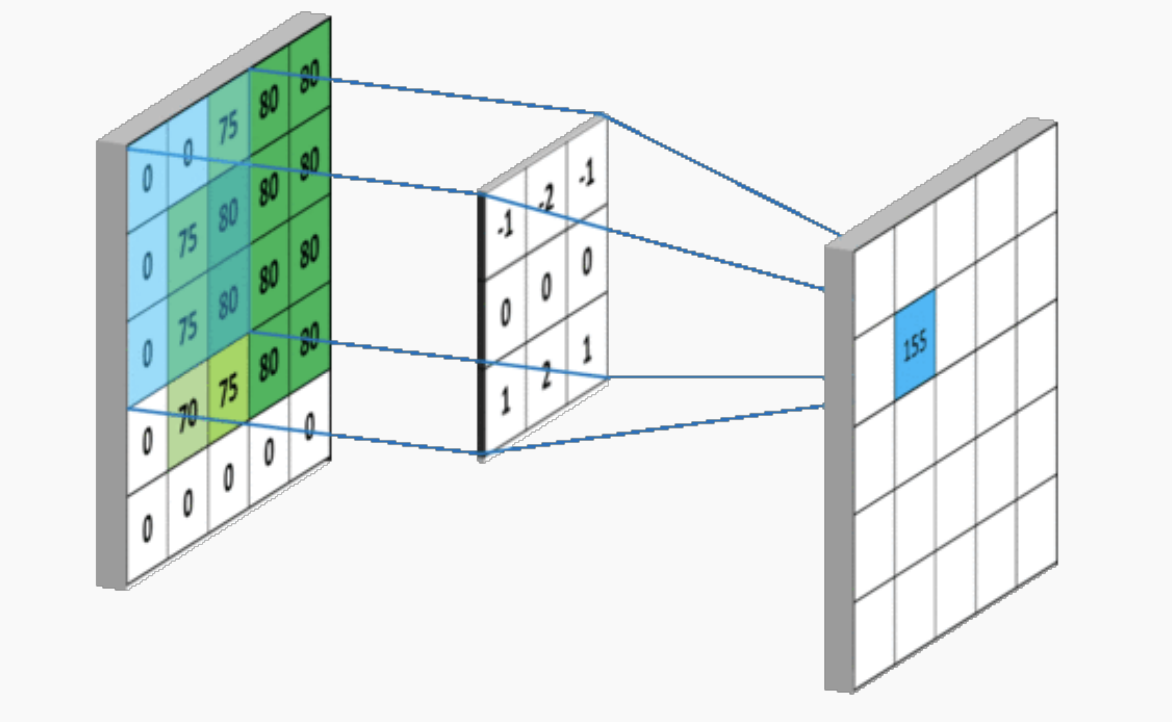
\includegraphics[width=0.9\textwidth]{convolution.png}
    \end{minipage}
    \begin{minipage}{0.49\textwidth}
        \centering
        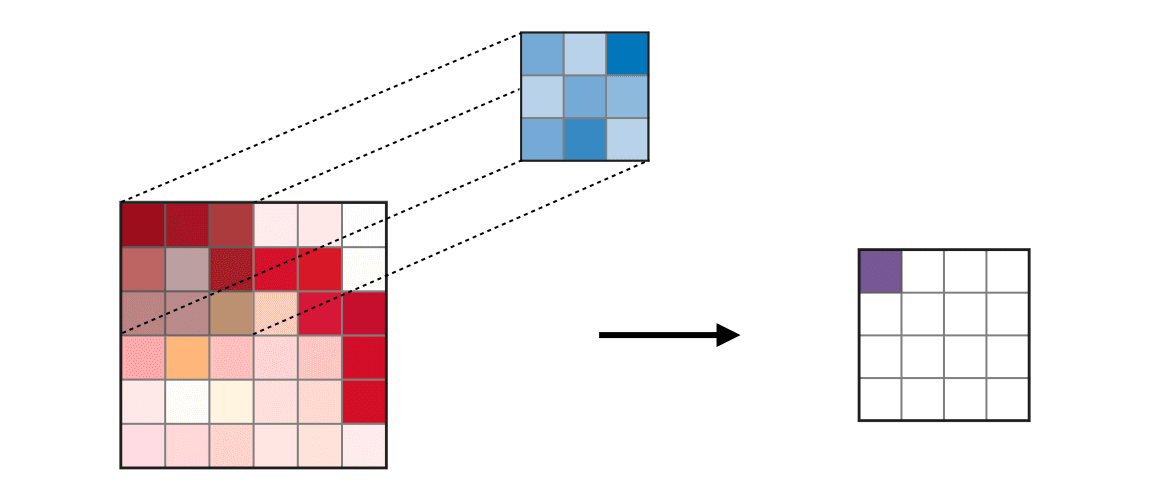
\includegraphics[width=0.9\textwidth]{convolution-layer-a.png}
    \end{minipage}  
    \caption{Faltung des Inputs mit einer Filter Matrix,
    Quellen: \cite{researcherSimpleIntroductionConvolutional2019}
    und \cite{amidiSuperVIPCheatsheet2019}}
    \label{fig:faltung}
\end{figure}
\vspace{1cm}

Jedes Faltungsergebnis, ergibt einen Wert für 
die nächste Schicht, die dadurch 
ein Korrelationsverhältnis zwischen
Filter Matrix und Input Bild erhält.
So werden, in den Filtern definierte Muster, wie 
beispielsweise vertikale Linien, 
aus dem Inputbild herausextrahiert und in 
den Folgeschichten, als sogenannte \Glspl{featuremap}
abgebildet.
\vspace{1cm}

\begin{equation}
    \label{eq:faltung}
    \begin{pmatrix}
        10 & 10 & 10 & 0 & 0 & 0\\
        10 & 10 & 10 & 0 & 0 & 0\\
        10 & 10 & 10 & 0 & 0 & 0\\
        10 & 10 & 10 & 0 & 0 & 0\\
        10 & 10 & 10 & 0 & 0 & 0\\
        10 & 10 & 10 & 0 & 0 & 0
    \end{pmatrix}
    \times
    \begin{pmatrix}
        1 & 0 & -1\\
        1 & 0 & -1\\
        1 & 0 & -1
    \end{pmatrix}
    = 
    \begin{pmatrix}
        0 & 30 & 30 & 0\\
        0 & 30 & 30 & 0\\
        0 & 30 & 30 & 0\\
        0 & 30 & 30 & 0
    \end{pmatrix}
\end{equation}
\vspace{0.5cm}
\begin{figure}[H]
    \centering
    \def\svgwidth{0.6\textwidth}
    \input{Bilder/convolution_graphical_all.pdf_tex}
    \caption{Faltung mit Filtermatrix zur Erkennung vertikaler Linien}
    \label{fig:faltung3}
\end{figure}

In Gleichung \ref{eq:faltung} ist beispielhaft die Faltung 
eines Inputbildes mit einem Filter, zur Erkennung 
vertikaler Linien, dargestellt. Da pro Zeile 
vier Faltungen angewendet werden, entsteht 
eine $4\times4$ Matrix. Soll die Ausgangsgröße 
(hier $6\times6$) beibehalten werden, kann
\textit{\Gls{zeropadding}} verwendet werden.
Durch die Faltung entsteht eine räumliche 
Invarianz für das zu erkennende Objekt im 
Input Bild.

Den \textit{Convolutional Layern} folgen meist
\textit{Pooling Layer}, zum \Gls{downsampling},
und eine ReLU-Aktivierungsfunktion.

Beim Pooling wird eine bestimme Anzahl an Werten 
zusammengefasst, indem entweder das Maximum oder der 
Mittelewert dieser Werte verwendet werden.

Durch hintereinanderschaltung mehrerer solcher
\textit{Convolutional Blöcke},
können in jeder Schicht immer komplexere Muster aus dem 
Inputbild herausextrahiert werden.

Die Features des Letzten \textit{Convolutional Layers}
 werden dann einem 
\textit{Fully Connected Layer}  zur Klassifikation 
übergeben, wie in Abbildung \ref{fig:lenet} anhand des 
ersten, von Yann LeCun entworfenen, \Glspl{cnn} zu erkennen ist.
\vspace{1cm}

\begin{figure}[H]
    \centering
    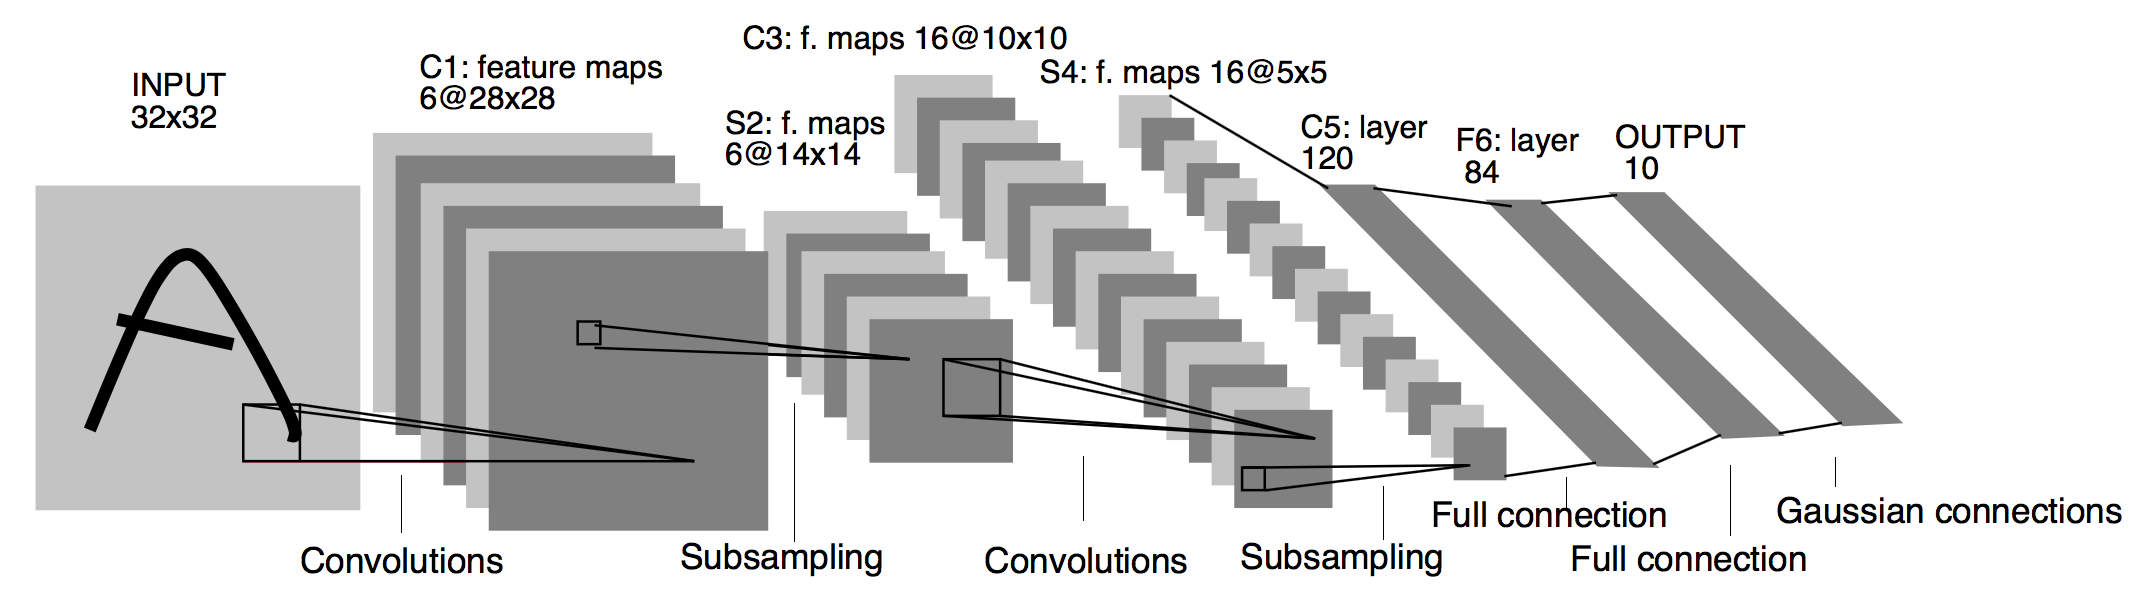
\includegraphics[width=\columnwidth]{lenet.png}
    \caption{LeNet-5 Architektur
    \cite{lecunGradientBasedLearningApplied1998}}
    \label{fig:lenet}
\end{figure}
\vspace{1cm}

Ein wesentlicher Vorteil gegenüber einem reinen 
\textit{Feedforward Network} ist, dass 
durch die gemeinsame Nutzung von Parametern, 
durch die Filter, ein geringerer Rechenaufwand entsteht.

Die Werte der Filter Matrizen, welche die zu 
extrahierenden Muster darstellen, 
werden über die \textit{Backpropagation} eingelernt.

Da die Merkmale, insbesondere in den vorderen 
\textit{Convolutional Layern}, für die meisten 
Klassen sehr ähnlich sind,
werden häufig Modelle mit vortrainierten Filtern 
verwendet.

Durch das sogenannte \textit{Transfer Learning}
müssen die Gewichte dann nur noch leicht, 
für den eigenen Datensatz, angepasst werden.



\subsection{Architkturen}\label{subsubsec:architectures}

Nachdem 1998 das erste \Gls{cnn} (Abbildung \ref{fig:lenet})
 von Yann LeCun in 
\cite{lecunGradientBasedLearningApplied1998} 
vorgestellt wurde, gab es eine Vielzahl 
an Weiterentwicklungen, welche genauere und 
effizientere Modelle hervorbracheten.

Gemessen und verglichen werden die Ergebnisse häufig an 
der \textit{Large Scale Visual Recognition Challenge (ILSVRC)}
\cite{ImageNetLargeScale}.
 
Namhafte Modelle, welche die Challenge in den letzten 
Jahren gewinnen konnten sind unter \cite{stanfordConvNetList}
zu finden und im Folgenden aufgelistet.

\begin{itemize}
    \item \textbf{AlexNet}, (2012), von Alex Krizhevsky 
        \cite{krizhevskyImageNetClassificationDeep2017b} besitzt eine 
        ähnliche Struktur wie LeCuns \textit{LeNet},
        ist jedoch Tiefer und besitzt mehrere \textit{Convolutional
         Layer} am Stück hintereinander,
        wodurch die Genauigkeit erhöht wurde.

    \item \textbf{ZF Net}, (2013), von Matthew Zeiler and Rob Fergus,
        \cite{zeilerVisualizingUnderstandingConvolutional2013}
        konnte das \textit{AlexNet} durch eine Vergrößerung der 
        mittleren \textit{Convolutional Layer}
        und eine Verkleinerung der Filter in den vorderen
        Schichten weiter optimieren.

    \item \textbf{VGGNet}, (2014), von Karen Simonyan and Andrew Zisserman
        \cite{simonyanVeryDeepConvolutional2015}.
        Dieses Modell zeigte, dass ein tieferes Netz
         (16 bis 19 \textit{Convolutional Layer})
        mit reduzierter Filter größe ($3\times3$) bessere
        Ergebnisse erzielt.    

    \item \textbf{GoogleLeNet}, auch bekannt als \textit{Inception}, (2014),
        von Szegedy et al \cite{szegedyGoingDeeperConvolutions2014},
        konnte mit den \textit{Inception Modulen},
        welche im Folgenden genauer erläutert werden, die Zahl der 
        Parameter, und dadurch den Rechenaufwand, deutlich veringern.

    \item \textbf{ResNet}, (2015) von Kaiming He et al 
        \cite{heDeepResidualLearning2015}, enthällt 
        als Erweiterung die \textit{Residual Blöcke}, in denen auf
        das Ergebnis eines Bocks zusätzlich der unveränderte
        Input Wert addiert wird.
\end{itemize}



\subsubsection{GoogleLeNet (Inception)}

Die Entwicklung der \Gls{cnn} Architekturen hat gezeigt,
dass sich durch Hinzufügen weiterer Schichten, sowie
der Verwendung einer größeren Anzahl an Neuronen je Schicht, 
die Genauigkeit verbessern lässt.
Das bringt jedoch auch die Nachteile eines 
größeren Rechenaufwands sowie der erhöhten 
Gefahr des \Glspl{overfitting} mit sich.

Das in \cite{szegedyGoingDeeperConvolutions2014} 
vorgestellte \textit{GoogleLeNet}, hat mit den in 
Abbildung \ref{fig:incept_modul} dargestellten
\textit{Inception Modulen}, einen neuen, 
effizienteren, Ansatz gefunden, die 
Komplexität und damit die Genauigkeit eines 
CNNs zu erhöhen.

Die Module bestehen aus parallel ausgeführten 
\textit{Convolutional Layern} mit den 
unterschiedlichen Filtergrößen $1\times1$,
 $3\times3$ und $5\times5$ welche 
am ende des Moduls über eine \textit{Filter 
concatenation} wieder zusammengeführt werden.
Zur Dimensionsreduktion werden, wie in 
Abbildung \ref{fig:incept_modul} dargestellt,
diesen Filtern noch $1\times1$ Filter vorgeschaltet.
Durch die Inception Module kommt das Modell, 
für gleiche Ergebnisse, mit deutlich weniger 
Parametern aus, als ein Modell ohne die Module.
Ein weiterer Vorteil ist, das durch die 
unterschiedlichen Filtergrößen, Merkmale 
unterschiedlicher skalierungen besser gefunden 
werden können.

Um die Effizienz weiter zu Steigern, wurden in 
der zweiten Version des \textit{GoogleLeNet}, beschrieben in
\cite{szegedyRethinkingInceptionArchitecture2015},
neben anderen Verbesserungen, die 
$5\times5$ Filter, jeweils durch zwei $3\times3$ Filter, 
ersetzt, was in Abbildung \ref{fig:incept_modul2}
dargestellt ist.
\vspace{1cm}

\begin{minipage}{0.45\textwidth}
    \centering
    


\tikzset{
    block/.style={
        rectangle,
        draw=black,
        fill=blue!20,
        minimum width=3em,
        minimum height=2em,
        text centered,
        node distance=5em
    },
    arrow/.style={
        draw,
        %thick,
        >=latex,
        ->
    }
}



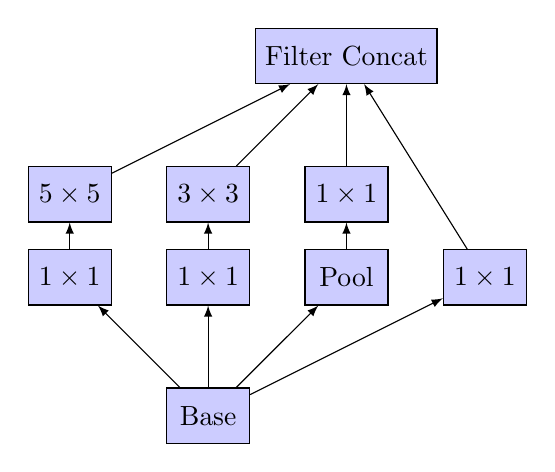
\begin{tikzpicture}[node distance=1.6cm]

    \node (concat) [block] {Filter Concat};

    \node (211) [block, below of=concat] {$1\times1$};
    \node (233) [block, left of=211] {$3\times3$};
    \node (255) [block, left of=233] {$5\times5$};


    \node (pool) [block, below of=211, node distance=3em] {Pool};

    \node (1111) [block, left of=pool] {$1\times1$};
    \node (1112) [block, left of=1111] {$1\times1$};
    \node (1113) [block, right of=pool] {$1\times1$};

    \node (base) [block, below of=1111] {Base};

    
    \draw[arrow] (base) -- (1111);
    \draw[arrow] (base) -- (1112);
    \draw[arrow] (base) -- (pool);
    \draw[arrow] (base) -- (1113);

    \draw[arrow] (pool) -- (211);
    \draw[arrow] (1111) -- (233);
    \draw[arrow] (1112) -- (255);
    \draw[arrow] (1113) -- (concat);

    \draw[arrow] (255) -- (concat);
    \draw[arrow] (233) -- (concat);
    \draw[arrow] (211) -- (concat);

    

\end{tikzpicture}

    \captionof{figure}{Inception Module der 1. Version}
    \label{fig:incept_modul}
\end{minipage}
\begin{minipage}{0.1\textwidth}
    \hfill
\end{minipage}
\begin{minipage}{0.45\textwidth}
    \centering
    
\tikzset{
    block/.style={
        rectangle,
        draw=black,
        fill=blue!20,
        minimum width=3em,
        minimum height=2em,
        text centered,
        node distance=5em
    },
    arrow/.style={
        draw,
        >=latex,
        ->
    }
}



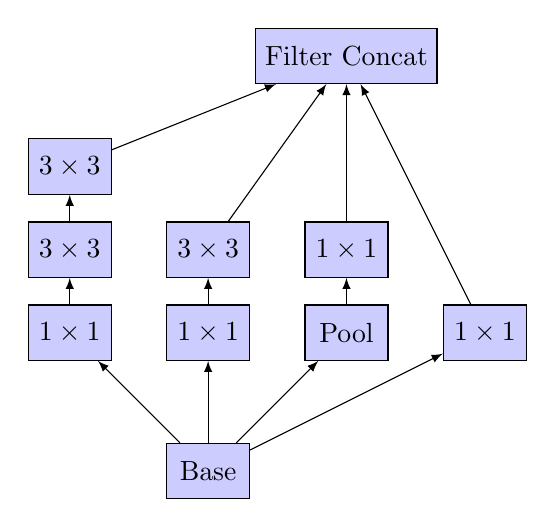
\begin{tikzpicture}[node distance=1.6cm]

    \node (concat) [block] {Filter Concat};

    \node (211) [block, below of=concat, node distance=7em] {$1\times1$};
    \node (233) [block, left of=211] {$3\times3$};
    \node (255) [block, left of=233] {$3\times3$};

    \node (333) [block, above of=255, node distance=3em] {$3\times3$};

    \node (pool) [block, below of=211, node distance=3em] {Pool};

    \node (1111) [block, left of=pool] {$1\times1$};
    \node (1112) [block, left of=1111] {$1\times1$};
    \node (1113) [block, right of=pool] {$1\times1$};

    \node (base) [block, below of=1111] {Base};

    
    \draw[arrow] (base) -- (1111);
    \draw[arrow] (base) -- (1112);
    \draw[arrow] (base) -- (pool);
    \draw[arrow] (base) -- (1113);

    \draw[arrow] (pool) -- (211);
    \draw[arrow] (1111) -- (233);
    \draw[arrow] (1112) -- (255);
    \draw[arrow] (1113) -- (concat);

    \draw[arrow] (255) -- (333);
    \draw[arrow] (333) -- (concat);
    \draw[arrow] (233) -- (concat);
    \draw[arrow] (211) -- (concat);

    

\end{tikzpicture}
    \captionof{figure}{Inception Module der 2. Version}
    \label{fig:incept_modul2}
\end{minipage}

\newpage
\subsubsection{Mobilenet}
Das MobileNet \cite{howardMobileNetsEfficientConvolutional2017a}
wurde mit dem Ziel geschaffen, durch eine geringere 
Komplexität, für Mobile Endgeräte oder Embedded-Anwendungen 
geeignet zu sein.

Dafür wurden die üblichen \textit{Convolutional Layer}
mit sogenannten \textit{Depthwise Seperable 
Convolutions} ersetzt, welche die Faltung in zwei separaten 
Schichten ausführt. Zuerst wird eine \textit{Depthwise  
Convolutions} auf die drei Farbkanäle getrennt ausgeführt.
Anschließend führt eine \textit{pointwise convolution}
mit $1\times1$ Filter diese wieder zusammen.


In der zweiten version des MobileNet
\cite{sandlerMobileNetV2InvertedResiduals2019},
wurden die \textit{Depth-wise Separable Convolutions}
wie folgt abgeändert:

Zuerst wird eine $1\times1$ Convolution mit ReLU
Aktivierungsfunktion ausgeführt, anschließend die 
\textit{Depthwise Convolutions}, gefolgt 
von einer weiteren $1\times1$ mit linearer 
Aktivierungsfunktion.


Desweiteren soll wie beim \textit{ResNet} eine 
\textit{residual connection}, welche Ein- mit
Ausgabewert eines Blocks verbindet, 
den Gradientenfluss unterstützen, wie in Abbildung 
\ref{fig:mobilenetv2} dargestellt ist.
\vspace{1cm}

\begin{figure}[H]
    \centering
    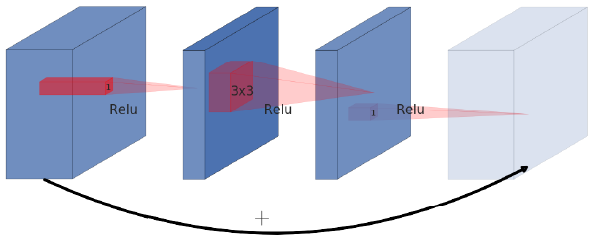
\includegraphics[width=0.7\textwidth]{mobilenet_v2.png}
    \caption{Residual block des MobilenetV2
    \cite{mobilenetv2Bild}}
    \label{fig:mobilenetv2}
\end{figure}


%---------------- SUBSECTION: Obj Detection ----------------
\subsection{Objekterkennung}\label{subsec:objdet_det}

Neben der Information, was sich auf einem Bild befindet, 
soll bei der Objekterkennung zusätzlich herausgefunden werden, 
wo sich das erkannte Objekt in dem Bild befindet.
In Abbildung \ref{fig:class_vs_det} wird der Unterschied 
veranschaulicht. Im linken Bild (Klassifikation) 
reicht es aus, dass das Modell das Vorhandensein einer Katze
im Bild, mit einer bestimmten Wahrscheinlichkeit, Schätzen kann,
im rechten Bild (Objekterkennung), soll das Modell, 
in Form von \textit{Bounding Boxen}, auch eine 
Lokalisierung vornehmen.

\vspace{1cm}
\begin{minipage}{0.5\textwidth}
    \centering
    Classification
\end{minipage}
\begin{minipage}{0.5\textwidth}
    \centering
    Detection
\end{minipage}
\begin{figure}[H]
    \centering
    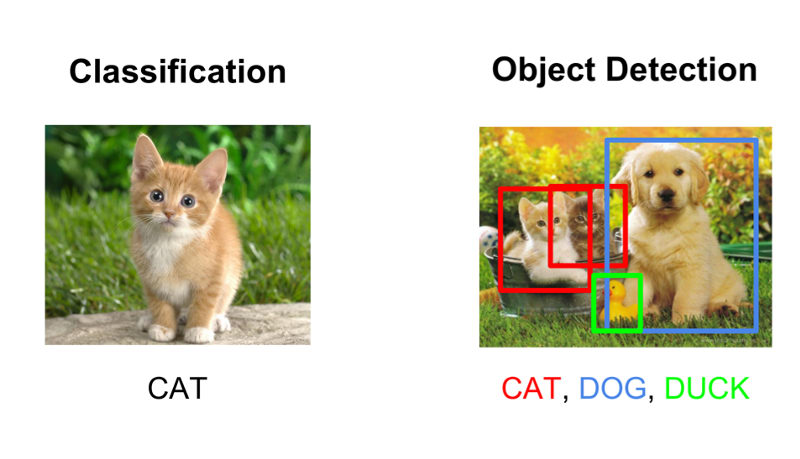
\includegraphics[width=0.8\textwidth]{classification_detection.jpeg}
    \caption{Unterschied: Klassifikation - Objekterkennung, 
    Quelle: \cite{ouaknineReviewDeepLearning2018a}}
    \label{fig:class_vs_det}
\end{figure}
\vspace{1cm}

Dafür wird die \Gls{cnn} Architektur so erweitert,
dass dem Modell für das Training neben den Klassen-Labels
auch die Koordinaten der \textit{Bounding Boxen},
welche das Objekt umrahmen, mit übergeben werden.

Diese können dann, mittels Regressionsverfahren, 
durch Annäherung der geschätzten an die richtigen 
Koordinaten, gelernt werden.

Bei den Verfahren zur Objekterkennung gibt es 
verschiedene Ansätze, die alle ein Basis-\Gls{cnn},
zur \textit{Feature Extraction} verwenden.
Die Lokalisierung findet über eine 
Vorschlagsgenerierung statt, welche aus 
Regionen im Input Bild besteht, die 
am wahrscheinlichsten ein Objekt enthalten.


%------------------- SECTION: Hardware ----------------------
\section{Neural Compute Stick 2}\label{ncs2}

Da das Training und die Inferenz von Deep Learning Algorithmen
sehr rechenintensiv ist, werden entsprechen leistungsfähige 
Prozessoren benötigt. Dabei ist die Ausführung auf einer
\Gls{gpu} meist effizienter als auf einer \Gls{cpu}.

Anwendungen die auf eingebetteten Systemen oder einplatinen 
Computern wie dem \textit{Raspberry Pi} laufen,
kommen dabei schnell an die Grenzen.

Eine Möglichkeit, dieses Problem zu umgehen,
ist es, die Bilddaten für die 
Verrechnung an eine Cloud zu senden, wo sie 
von einem leistungsstärkeren Rechner inferiert und 
dann wieder zurückgesendet werden.

Sollen die Daten, wie es beim \textit{Edge Computing} der Fall ist, 
auf dem Anwendungsgerät direkt verarbeitet werden,
gibt es speziell für die Inferenz von Deep Learing Algorithmen
geeignete Hardware.
Durch Fokus auf hohe Parallelität, anstatt schneller Taktrate
bei den Berechnungen, können solche Prozessoren
Deep Learning spezifische Rechenoperationen, 
wie z.B. die Matrixmultiplikation, besonders effizient 
ausführen.

Die Inferenzbeschleunigende Hardware kann dabei entweder
als eigenständiges \textit{\Gls{soc}}
System wie z.B. der \textit{Nvidia Jetson TX2} agieren, oder
in Verbindung mit einem \textit{Host Pc}, wie der, in der Arbeit 
verwendete, \textit{Neural Compute Stick 2} (NCS2) von \textit{Intel}.

Der in Abbildung \ref{fig:ncs2} gezeigte NCS2
verwendet für die Inferenz eine
\textit{Movidius Myriad X} \Gls{vpu},
welche in Abbildung \ref{fig:myriad} schematisch 
dargestellt ist.

Diese besteht, wie in
\cite{haussermannFunktionUndEffizienz} genauer 
beschrieben ist, aus der Neural Compute Engine, 
zur beschleunigten Berechnung Neuronaler Netze,
einem Bildbeschleuniger, 16 SHAVE Prozessoren, einem 
Bildsignalprozessor sowie einem RISC CPU Core.

\vspace{1cm}
\begin{minipage}{0.4\textwidth}
    \centering
    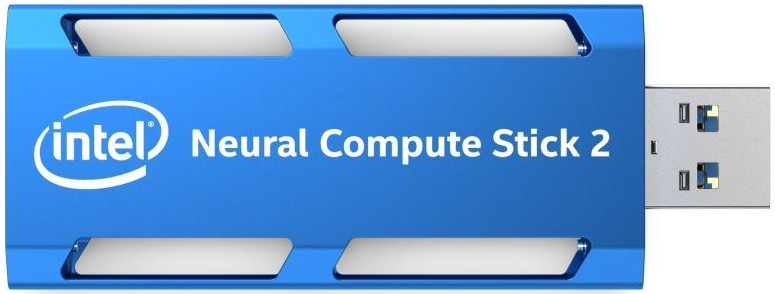
\includegraphics[width=\textwidth]{ncs2_top.jpg}
    \captionof{figure}{NCS2, \cite{ncs2}}
    \label{fig:ncs2}
\end{minipage}
\begin{minipage}{0.6\textwidth}
    \centering
    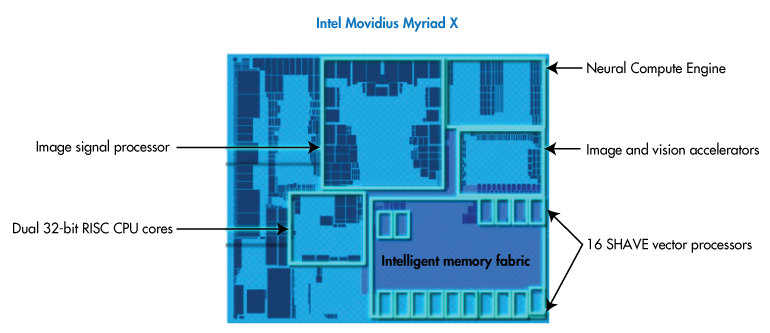
\includegraphics[width=\textwidth]{myriad.png}
    \captionof{figure}{Myriad Chip,
    \cite{IntelMyriadVision}}
    \label{fig:myriad}
\end{minipage}


\subsection{OpenVino Toolkit}

Zur Ausführung der Inferenz, eines trainierten Deep Learing
Modells, auf dem NCS2, wird das Toolkit 
\textit{OpenVino} von Intel verwendet.
Dieses ist eine Software Plattform zur Otimierung und Inferenz 
von \Gls{cnn}-basierten Modellen auf verschiedener Intel Hardware.

Dabei wird ein eigenes Dateiformat für die Modelle verwendet, 
die \textit{Intermediate Representation} (IR),
welche die Struktur des Modells 
in einer Xml-Datei und die trainierten Gewichte in 
einer Binärdatei definiert.
Mit dem \textit{Model Optimizer} des Toolkits,
können Modelle, welche in den den \Glspl{framework} \textit{TensorFlow,
Caffe, ONNX, Kaldi,} oder \textit{MXNET} trainiert wurden, 
in das IR-Format konvertiert werden.

Um diese dann auf die entsprechende Hardware zu laden und anwendbar 
zu machen, wird die auch in \textit{OpenVino} enthaltene
\textit{InferenceEngine} verwendet.
Diese bietet eine \Gls{api}, mit der aus der Anwendung
 heraus, in den Programmiersprachen C++ oder Python,
  auf die Funktionen der 
\textit{InferenceEngine} zugegriffen werden können.


In Abbildung \ref{fig:openvinoflow} ist der Workflow mit 
\textit{Openvino}, welcher das Training eines
 Deep Learning Modells mit der Implementierung
  einer Nutzer Anwendung verbindet, 
dargestellt.


\vspace{1cm}
\begin{figure}[H]
    \centering
    \def\svgwidth{0.8\textwidth}
    \input{Bilder/open_vino_workflow_neu.pdf_tex}
    \caption{OpenVino Workflow, angelent an 
    \cite{openvinoflow}}
    \label{fig:openvinoflow}
\end{figure}
